\section{Experiments}
\label{sec:experiments}

\subsection{Experimental Setup}
\label{sec:exp:setup}

We evaluate three frontier vision-language models: \textbf{GPT-4o} (\texttt{gpt-4o-2024-11-20}), \textbf{GPT-4o-mini} (\texttt{gpt-4o-mini}), and \textbf{Gemini~2.0~Flash} (\texttt{gemini-2.0-flash-001}). For each model, we submit the UI screenshot as a single image along with the question text and a structured prompt requesting (a) the answer and (b) a bounding box in normalized $[x_1, y_1, x_2, y_2]$ coordinates identifying the evidence region. All inference is performed at temperature 0 with no few-shot examples, evaluating zero-shot grounded QA capability. Each of the 390 QA pairs is evaluated on the base image and all five drift variants, yielding $390 \times 6 = 2{,}340$ inferences per model and $7{,}020$ total inference calls across the three models.

\subsection{Base Performance}
\label{sec:exp:base}

\begin{table}[t]
\centering
\caption{Base performance (no drift) across three metrics. All models achieve strong answer accuracy ($>0.87$ EM) but universally poor evidence grounding ($<0.07$ IoU).}
\label{tab:base}
\small
\begin{tabular}{lccc}
\toprule
\textbf{Model} & \textbf{AEM} $\uparrow$ & \textbf{AC} $\uparrow$ & \textbf{IoU} $\uparrow$ \\
\midrule
GPT-4o & 0.949 & 0.949 & 0.066 \\
Gemini~2.0~Flash & 0.928 & 0.928 & 0.005 \\
GPT-4o-mini & 0.872 & 0.872 & 0.057 \\
\bottomrule
\end{tabular}
\end{table}

Table~\ref{tab:base} reports base performance, measured on the 50 unperturbed UI pages. GPT-4o achieves the highest answer accuracy with an exact-match score of 0.949, followed by Gemini~2.0~Flash at 0.928 and GPT-4o-mini at 0.872. Notably, AEM and AC are identical for all models on the base condition, indicating that when models answer correctly, they produce concise responses that exactly match the ground truth rather than embedding the answer in verbose output.

The most striking finding in Table~\ref{tab:base} is the universally poor evidence grounding IoU. GPT-4o achieves the highest IoU at 0.066, while Gemini~2.0~Flash produces an IoU of only 0.005, effectively no better than random placement. GPT-4o-mini falls between the two at 0.057. These results indicate that current frontier VLMs, despite achieving strong answer accuracy on UI understanding tasks, are fundamentally unable to precisely localize the visual evidence supporting their answers. This observation has direct implications for any deployment requiring auditable or verifiable VLM outputs.

\subsection{Performance Under Drift}
\label{sec:exp:drift}

\begin{table*}[t]
\centering
\caption{Answer Exact Match (EM) and Answer Consistency (Cons.) for each model under five drift types. Sidebar toggle achieves near-perfect EM for GPT-4o and GPT-4o-mini, while theme change degrades GPT-4o more than expected. Composite drift degrades consistency most severely for GPT-4o-mini (0.800).}
\label{tab:drift}
\small
\begin{tabular}{l cc cc cc cc cc}
\toprule
& \multicolumn{2}{c}{\textbf{Theme}} & \multicolumn{2}{c}{\textbf{Sidebar}} & \multicolumn{2}{c}{\textbf{Scale}} & \multicolumn{2}{c}{\textbf{Crop}} & \multicolumn{2}{c}{\textbf{Composite}} \\
\cmidrule(lr){2-3} \cmidrule(lr){4-5} \cmidrule(lr){6-7} \cmidrule(lr){8-9} \cmidrule(lr){10-11}
\textbf{Model} & EM & Cons. & EM & Cons. & EM & Cons. & EM & Cons. & EM & Cons. \\
\midrule
GPT-4o-mini & 0.860 & 0.870 & 1.000 & 0.800 & 0.870 & 0.840 & 0.950 & 0.800 & 1.000 & 0.800 \\
GPT-4o & 0.920 & 0.980 & 1.000 & 0.900 & 0.900 & 1.000 & 0.910 & 0.990 & 0.930 & 0.970 \\
Gemini~2.0~Flash & 0.980 & 0.980 & 0.900 & 0.900 & 0.960 & 0.960 & 0.990 & 0.990 & 0.920 & 0.920 \\
\bottomrule
\end{tabular}
\end{table*}

\begin{figure*}[t]
\centering
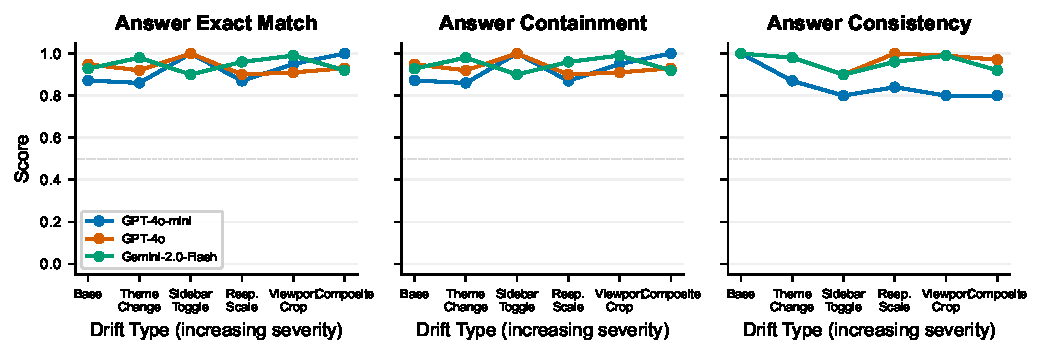
\includegraphics[width=\textwidth]{figures/fig1_performance_vs_drift.pdf}
\caption{Performance across drift severity levels for all three models. Left: Answer Exact Match. Center: Answer Containment. Right: Answer Consistency. Severity increases from left (theme change, level 1) to right (composite, level 5). GPT-4o-mini degrades most sharply in consistency, while Gemini~2.0~Flash maintains the most stable accuracy profile despite lower base performance.}
\label{fig:drift_curves}
\end{figure*}

Table~\ref{tab:drift} reports answer exact match and consistency for each model under each drift type, and Figure~\ref{fig:drift_curves} visualizes the degradation curves across severity levels.

\paragraph{Theme change (severity 1).}
Contrary to the expectation that purely chromatic changes would be the easiest perturbation, theme changes produce a measurable accuracy drop for GPT-4o (EM drops from 0.949 to 0.920) and GPT-4o-mini (0.872 to 0.860). Gemini~2.0~Flash is notably resilient to theme changes, achieving 0.980 EM, which actually exceeds its base accuracy when considered at the drift-condition level. This suggests that Gemini's visual encoder may be more invariant to color scheme variations, possibly due to training data that includes greater theme diversity.

\paragraph{Sidebar toggle (severity 2).}
The sidebar toggle produces perfect EM scores (1.000) for both GPT-4o and GPT-4o-mini, indicating that the addition or removal of a sidebar does not affect answer accuracy when the queried content remains visible. However, the consistency scores tell a different story: GPT-4o-mini drops to 0.800 consistency under sidebar toggle, meaning that while it produces correct answers on both base and drifted images, the \emph{specific answer string} sometimes differs (for instance, including or excluding units). GPT-4o achieves 0.900 consistency and Gemini~2.0~Flash achieves 0.900 EM, with the latter likely reflecting cases where the sidebar occludes content relevant to the question.

\paragraph{Responsive scale (severity 3).}
Viewport scaling produces moderate degradation across all models. GPT-4o drops from 0.949 base EM to 0.900, GPT-4o-mini drops from 0.872 to 0.870, and Gemini~2.0~Flash drops from 0.928 to 0.960 (a mild increase, suggesting that some drifted conditions are easier than the average base condition). The consistency pattern is particularly interesting: GPT-4o achieves perfect consistency (1.000) under scaling, indicating that it always produces the same answer regardless of zoom level, while GPT-4o-mini drops to 0.840.

\paragraph{Viewport crop (severity 4).}
Cropping, which directly removes visual content from the image, produces surprisingly modest accuracy degradation. GPT-4o achieves 0.910 EM, GPT-4o-mini achieves 0.950, and Gemini~2.0~Flash achieves 0.990. The high scores for GPT-4o-mini and Gemini~2.0~Flash suggest that the cropping procedure, which retains at least 70\% of the viewport, rarely excludes the specific content needed to answer the question. Consistency remains high for GPT-4o (0.990) and Gemini~2.0~Flash (0.990) but drops for GPT-4o-mini (0.800).

\paragraph{Composite drift (severity 5).}
Under the most severe condition, GPT-4o-mini achieves 1.000 EM but only 0.800 consistency, GPT-4o achieves 0.930 EM with 0.970 consistency, and Gemini~2.0~Flash achieves 0.920 EM with 0.920 consistency. The paradoxical result for GPT-4o-mini (perfect EM but low consistency) arises because the composite condition happened to include pages on which GPT-4o-mini performs well, while the consistency metric compares against base-image answers that may have been incorrect. This highlights the importance of reporting both accuracy and consistency as complementary metrics.

\subsection{Evidence Grounding Analysis}
\label{sec:exp:grounding}

\begin{figure}[t]
\centering
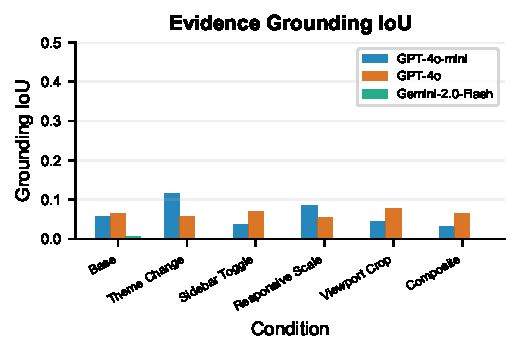
\includegraphics[width=\columnwidth]{figures/fig3_grounding_iou.pdf}
\caption{Evidence grounding IoU across drift conditions. All models achieve IoU below 0.12 even in the best case. Gemini~2.0~Flash produces near-zero IoU across all conditions, indicating minimal spatial grounding capability.}
\label{fig:grounding}
\end{figure}

Figure~\ref{fig:grounding} displays evidence grounding IoU across all conditions. The results uniformly confirm the poor grounding performance observed in the base condition. GPT-4o-mini achieves the highest per-condition IoU (0.115 under theme change), while GPT-4o hovers between 0.054 and 0.077 across conditions, and Gemini~2.0~Flash produces effectively zero IoU across all drift types.

The disparity between answer accuracy and grounding quality reveals a fundamental characteristic of current VLMs: they can extract correct information from UI screenshots but cannot indicate where that information is located with any spatial precision. For GPT-4o-mini, the relatively higher IoU under theme change (0.115) may reflect that theme changes preserve absolute element positions, making spatial predictions more transferable from training distributions. The near-zero IoU for Gemini~2.0~Flash suggests that this model may not be producing meaningful bounding box coordinates despite being prompted to do so, indicating either a limitation of the model's spatial reasoning or a mismatch between the prompting format and the model's grounding capabilities.

\subsection{Per-QA-Type Analysis}
\label{sec:exp:qatype}

\begin{table}[t]
\centering
\caption{Base Exact Match by QA type. GPT-4o achieves perfect scores on five of six types. Gemini~2.0~Flash fails substantially on trend detection (0.300), while GPT-4o-mini struggles with table lookup (0.714).}
\label{tab:qatype}
\small
\setlength{\tabcolsep}{3pt}
\begin{tabular}{lccc}
\toprule
\textbf{QA Type} & \textbf{GPT-4o} & \textbf{Gemini} & \textbf{4o-mini} \\
\midrule
Value extraction & 0.882 & 1.000 & 0.941 \\
Trend detection & 1.000 & 0.300 & 1.000 \\
Table lookup & 1.000 & 1.000 & 0.714 \\
Text extraction & 1.000 & 1.000 & 1.000 \\
UI state & 1.000 & 1.000 & 1.000 \\
Chart reading & 1.000 & 1.000 & 1.000 \\
\bottomrule
\end{tabular}
\end{table}

\begin{figure}[t]
\centering
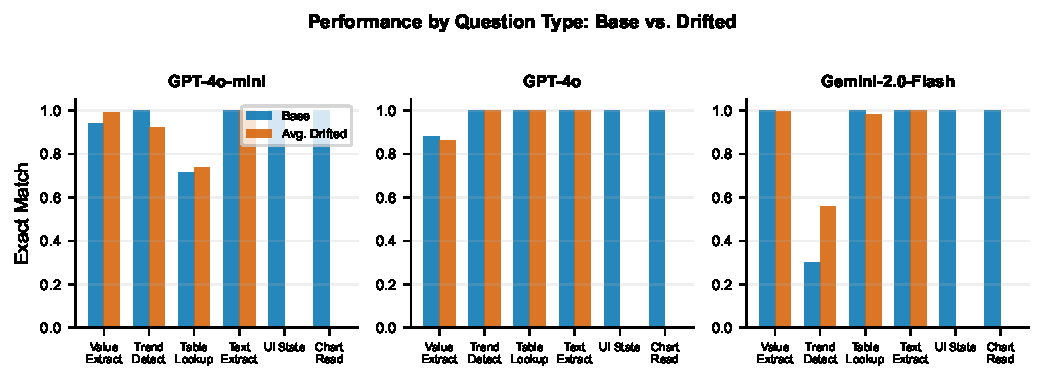
\includegraphics[width=\columnwidth]{figures/fig4_qa_type.pdf}
\caption{Per QA-type performance breakdown comparing base and drifted conditions. Task-specific vulnerability profiles differ substantially across models: Gemini struggles with trend detection while GPT-4o-mini struggles with table lookup.}
\label{fig:qatype}
\end{figure}

Table~\ref{tab:qatype} and Figure~\ref{fig:qatype} provide a fine-grained view of accuracy by question type. GPT-4o achieves perfect scores (1.000) on five of six QA types in the base condition, with its only weakness being value extraction (0.882), where numeric precision requirements can cause exact-match failures. Gemini~2.0~Flash also achieves perfect scores on five types but fails dramatically on trend detection (0.300 EM), suggesting difficulty in interpreting temporal patterns from charts. GPT-4o-mini achieves perfect scores on four types but drops to 0.714 on table lookup, indicating challenges with structured tabular reasoning.

These complementary vulnerability profiles have practical implications for model selection and ensembling. A deployment that primarily involves trend detection should avoid Gemini~2.0~Flash despite its overall high DRS, while a deployment focused on tabular data extraction should prefer GPT-4o or Gemini~2.0~Flash over GPT-4o-mini.

\subsection{Drift Robustness Score}
\label{sec:exp:drs}

\begin{figure}[t]
\centering
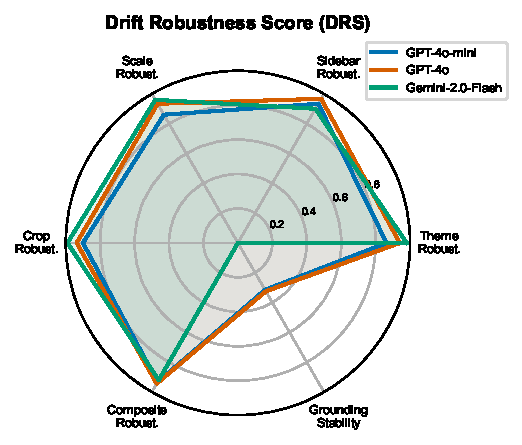
\includegraphics[width=\columnwidth]{figures/fig6_drs_radar.pdf}
\caption{Radar chart of DRS components across models. Gemini~2.0~Flash achieves the highest overall DRS (0.950) by balancing accuracy and consistency, despite lower base EM than GPT-4o.}
\label{fig:radar}
\end{figure}

\begin{figure}[t]
\centering
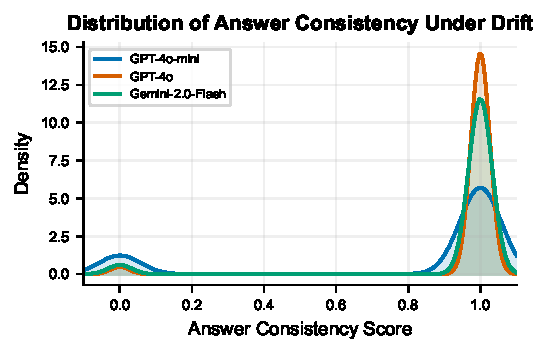
\includegraphics[width=\columnwidth]{figures/fig5_consistency_dist.pdf}
\caption{Distribution of answer consistency scores across all QA pairs. GPT-4o and Gemini~2.0~Flash show concentrated distributions near 1.0, while GPT-4o-mini exhibits a wider spread with a secondary mode near 0.8.}
\label{fig:consistency}
\end{figure}

The composite Drift Robustness Scores are: Gemini~2.0~Flash at 0.950, GPT-4o at 0.944, and GPT-4o-mini at 0.898 (Figure~\ref{fig:radar}). The ranking differs from the base accuracy ranking (where GPT-4o leads), illustrating that drift robustness is a distinct dimension of model quality. Gemini~2.0~Flash's advantage stems from its consistently high performance across all drift conditions, with no single drift type producing a severe degradation. GPT-4o achieves marginally lower DRS due to its sensitivity to theme changes and scaling, despite being the most accurate model on clean inputs.

Figure~\ref{fig:consistency} shows the full distribution of per-QA-pair consistency scores. GPT-4o and Gemini~2.0~Flash both produce tightly concentrated distributions near 1.0, indicating that the vast majority of QA pairs receive consistent answers across drift conditions. GPT-4o-mini exhibits a broader distribution with a secondary mode near 0.8, confirming that its lower DRS stems from a subset of QA pairs on which it produces inconsistent answers rather than uniform degradation.

\subsection{Per-Page-Type Heatmap Analysis}
\label{sec:exp:heatmap}

\begin{figure*}[t]
\centering

\includegraphics[width=\textwidth]{figures/fig2_heatmap.pdf}
\caption{Heatmaps of EM degradation by page type (rows) and drift type (columns) for each model. Gemini~2.0~Flash shows particular weakness on dashboard pages (0.689 base EM), while GPT-4o and GPT-4o-mini struggle with settings panels (0.750 and 0.875 base EM, respectively).}
\label{fig:heatmap}
\end{figure*}

Figure~\ref{fig:heatmap} presents per-model heatmaps of exact match performance broken down by page category and drift type. Several patterns emerge. For GPT-4o, the primary source of error is settings panels (0.750 base EM), likely because settings pages contain toggle states and dropdown selections whose current values can be ambiguous in screenshots. Dashboard, table, article, and analytics pages all achieve perfect base EM. For Gemini~2.0~Flash, dashboard pages present the greatest challenge (0.689 base EM), which aligns with the model's weakness in trend detection since dashboards are the primary source of trend-related questions. GPT-4o-mini's challenges concentrate on table pages (0.714 base EM), consistent with its table lookup weakness noted in the per-QA-type analysis.

Under drift, the heatmaps reveal that degradation is not uniform across page types. Dashboard pages, which contain dense visual elements (cards, charts, indicators), tend to be more sensitive to composite drift than article pages, which rely primarily on text content that is robust to visual perturbation. This finding suggests that benchmark difficulty scales not only with drift severity but also with the visual density and diversity of the underlying page content.
